
\vspace{-.2in}
\section{PROJECT ACHIEVEMENTS}
\vspace{-.2in}

Advanced fusion and fission energy are promising carbon-free resources capable of meeting global energy needs. Recent investments have spurred innovation in both fields, particularly in fusion. U.S.-based fusion companies like Commonwealth Fusion Systems \cite{cfs}, General Atomics \cite{ga}, Realta Fusion \cite{realta}, and Zap Energy \cite{zap} are pioneering various concepts, attracting support from notable investors such as Jeff Bezos \cite{general_fusion}. This private sector growth is a significant trend as academic research moves towards commercialization.

The design, certification, and licensing of novel energy concepts pose formidable hurdles due to the lack of large-scale test facilities, resulting in a severe deficit of relevant data. Developing appropriate models for full-system analysis requires {\em high-fidelity numerical simulations} and advanced instrumented experiments. Both fusion and fission systems involve complex multi-physics effects, which are challenging to unravel experimentally.

\textbf{\em Our objective is to illuminate multi-physics phenomena involving radiation transport, fluid flow, heat transfer, and magneto-hydrodynamics (MHD) in fusion systems.} Understanding these interactions is crucial for rapid commercialization of cost-competitive fusion products. A recent milestone at the National Ignition Facility saw a self-heated burning plasma achieve net energy gain \cite{nif}, sparking unprecedented enthusiasm for sustainable fusion concepts. However, a major challenge in deuterium-tritium (D-T) fusion is tritium fuel production, involving complex interactions between neutron activation, fluid flow, heat transfer, and MHD.

\begin{wrapfigure}{l}{0.4\textwidth}
\centering
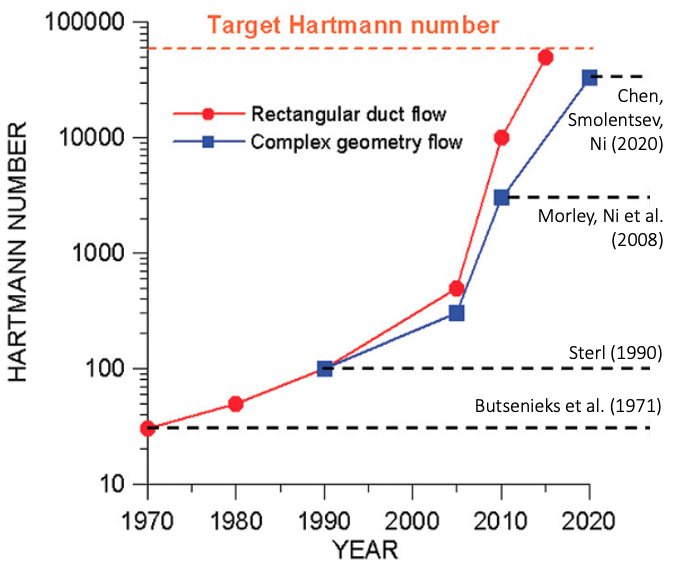
\includegraphics[width=0.95\textwidth]{figs/ha_history_mhd2.png}
\caption{\label{fig:mhd1} 
\small Historical limitations in MHD.}
\end{wrapfigure}

To accelerate fusion energy technology deployment, this project uses
NekRS~\cite{nekrs} and OpenMC~\cite{Romano2015}, with GPU acceleration, for
critical understanding and model development of whole-device multiphysics
phenomena. This effort will span three years on Frontier and Aurora platforms.
Both tools are developed under ECP projects targeting exascale platforms and
GPU computing, demonstrating exceptional performance. NekRS has shown
impressive capabilities, performing Large Eddy Simulation (LES) of a full core
in six hours using 27684 V100s on Summit~\cite{peb21}, and sustaining $>$28
PFLOPS performance on up to 9,000 nodes of Frontier. OpenMC recently achieved 3
million particles/sec per Sunspot node. This demonstrated performance has led
to deploying Nek5000/RS and OpenMC in the nuclear industry at companies such as
Kairos Power, Terrapower, and First Light Fusion.

\noindent{\textbf{\textit{Breeder Module Multiphysics }}}
Of the 33 concepts promoted by the Fusion Industry Association, 22 rely on a deuterium-tritium (D-T) fuel cycle \cite{tfi}. Tritium, with no meaningful natural abundance, is radioactive and extremely expensive, requiring significant online reprocessing for production, extraction, and reuse \cite{tanabe}.

Fusion devices using the D-T fuel cycle employ {\it breeder modules} to produce tritium. These modules, lining the plasma-facing surface, activate Li$^6$ (usually liquid lead-lithium) to produce tritium, which is then extracted for reuse. Breeder modules also extract heat for electricity generation and shield the vessel and magnets from radiation damage. {\it Achieving a breeder module design that satisfies these objectives is critical for commercializing fusion energy} \cite{tillack}. Magnetically-confined plasmas must consider MHD interactions, which introduce additional pressure losses scaling with magnetic field strength, requiring a balance between plasma confinement and pumping power.

Despite their importance, breeder modules' complex multiphysics in intricate geometries have been limited by prior computing power. Foundational design work often relied on geometric simplifications. Detailed modeling of MHD effects on blanket design is underway using codes such as HIMAG and MHD-UCAS~\cite{smolentsev2023}, but these are not yet capable of leveraging exascale computing for holistic modeling.  The challenges of modeling MHD are well represented in Figure~\ref{fig:mhd1}. We are conducting multiphysics simulations of breeder modules using OpenMC and NekRS, including heating from photon energy deposition, and considering validation through experimental facilities.

\vspace*{-.25in} \subsection{Significance of Accomplishments to Date}
\vspace*{-.20in}

\input tex/breeder
\input tex/chimera

\vspace{-.25in}
\subsection{Allocation Use}
\label{sec:usage2}
\vspace{-.2in}

Originally, we planned for the bulk of fusion simulations to be performed on Aurora, but the allocation was shifted to Frontier.
We have used all the allocation\ so far in 2024, exceeding 100 \%. This is because the scaling study we performed for CHIMERA was more expensive than originally thought. Moreover, we were given a smaller allocation than submitted (1 node hour on Frontier is not equivalent to our estimate of a node hour on Aurora).

Most of the allocation was spent on capability runs exceeding 50 \% of the machine by one user for CHIMERA. The remainder were smaller runs performed primarily by 6 users. 

We envision smaller allocation usage throughout the year primarily advancing the single breeder module calculations.

\input tex/readiness

\vspace{-.25in}
\section{PROJECT PLANS FOR NEXT YEAR} % typically about 6 pages
\vspace{-.2in}
\
Over the past decade, the Nuclear Energy Advanced Modeling and Simulation (NEAMS) program \cite{sofu2017us} has focused on developing advanced CFD software to support the deployment of advanced reactors. CFD is now widely used in reactor design and safety analysis \cite{roelofs2018thermal}, particularly for advanced reactors, where simulations complement experiments due to limited integral test data.

RANS \cite{conner2010cfd} and URANS are commonly used in industry and research for their reliability, but they have limitations in accuracy and turbulence modeling \cite{merzari2010numerical}. These models struggle with predicting turbulent fluctuations and high-order statistics \cite{yuan2017flow}.

Wall-resolved LES and DNS offer lower uncertainty and deeper insights into flow physics but have historically been limited by high computational costs \cite{grotzbach1999direct}. With advancements in petascale and pre-exascale computing, larger-scale simulations, including full-core SMRs, have become feasible \cite{merzari2017large,Fang2021}.

In our 2022 INCITE, we conducted full-core RANS CFD models of SMRs and SFRs, providing valuable thermal-fluid information. To enhance accuracy and resolve flow regimes affecting heat transfer in SMRs and SFRs, our 2024 proposal aims to include LES modeling of fuel bundles and mixing vanes. We also propose developing extensive datasets for multiphysics fusion applications.

\begin{displayquote}
\textit{
Building upon our extensive experience and recent achievements, this proposal seeks to develop high-fidelity datasets for fusion and fission applications. This includes first-of-a-kind full-core hybrid RANS-LES datasets to address knowledge gaps iin multiphysics simulations of breeder blankets.}
\end{displayquote}

We consider the velocity, continuity, and energy equations that
describe the constant-property incompressible flow of a Newtonian fluid:
\begin{equation}
\frac{\partial  u_i  }{\partial t} +  \frac{\partial}{\partial x_j} \left( u_i u_j \right) =-\frac{1}{\rho} \frac{\partial p}{\partial x_i} + \frac{\partial}{\partial x_j} \left[ \nu \left( \frac{\partial u_i}{\partial x_j} +\frac{\partial u_j}{\partial x_i} \right) \right]
+ f_i,
\hspace*{.3in}
\frac{\partial u_i}{\partial x_i} = 0
\label{eq:UEqn}
\end{equation}
\begin{equation}
\rho c_p \left( \frac{\partial T }{\partial t} + u_j \frac{\partial T}{\partial x_j} \right) = \frac{\partial }{\partial x_j} \left( \lambda \frac{\partial T}{\partial x_j} \right)
\label{eq:EEqn}
\end{equation}
where $u$ is the velocity, $p$ is the pressure, $T$ is the temperature, $\rho$
is the  density, $\nu$ is the kinematic viscosity, $\lambda$ is
the thermal conductivity, and $c_p$ is the heat capacity. In natural
convection cases, the Boussinesq or low Mach approximations
\cite{tomboulides1997numerical} are applied, leading to different
formulations available in Nek5000/RS. In the presence of an electromagnetic
field, additional source terms appear in the Navier-Stokes equations, which are
coupled to Maxwell's equations or MHD equations scaled with Alfven velocity
factors including Lorentz force in Eq.~(\ref{eq:UEqn}):
%
\begin{equation}
f_i = B_j \frac{\partial  B_i}{\partial x_j} 
\label{eq:MHDL}
\end{equation}
\begin{equation}
\frac{\partial  B_i  }{\partial t} +  \frac{\partial}{\partial x_j} \left( u_i B_j \right) = \frac{\partial }{\partial x_j} \left( B_j u_i \right) +  \nu_m \frac{\partial^2  B_i}{\partial x_j \partial x_j}, \hspace*{.5in}
\frac{\partial B_i}{\partial x_i} = 0
\label{eq:MHDB}
\end{equation}
Note that $\nu_m$ is magnetic diffusivity, B is magnetic field in units of Alfven velocity, and pressure $p$ becomes total pressure equal to $p_{hydro} + B^2/2$.
 %
{\it NekRS is the primary code that will be employed
in the MHD analysis.}

%We restrict our discussion to turbulence-resolving simulations such as DNS and
%wall-resolved LES. 
In advection-dominated problems such as the one described by
Eqs. (\ref{eq:UEqn})--(\ref{eq:EEqn}) at moderate to high Reynolds numbers, the
high-wavenumber component of transported quantities does not decay
exponentially, as observed in diffusion-dominated problems. Therefore, both
meaningful signals and numerical errors can persist in time, and appropriate
numerical schemes must be selected in order to avoid excessive dispersion.
The spectral element method, which is the basis for Nek5000/RS, is ideally
suited for this type of analysis. %We note that LES is usually performed within
%Nek5000/RS using an explicit filter \cite{schlatter21}.

For radiation transport, we consider coupled neutron-photon transport twith continuous-energy nuclear data and solved by the Monte Carlo method.
Statistics regarding average particle behavior are converged by simulating many individual particle histories,
providing a stochastic solution to the Boltzmann transport equation,
\begin{equation}
\label{eq:k_eigenvalue}
\frac{1}{v}\frac{\partial\psi}{\partial t}+\hat{\Omega}\cdot\nabla\psi+\Sigma_t\psi=\int_{4\pi}d\hat{\Omega}' \int_{0}^\infty  dE'\Sigma_s(E'\rightarrow E, \hat{\Omega}'\rightarrow\hat{\Omega})\psi+s
\end{equation}
where $v$ is the particle velocity, $\psi$ is the angular particle flux, $\hat{\Omega}$ is the unit solid angle, $\Sigma$ are various neutron interaction
probability cross sections, and $s$ is a source. For the fission applications in this proposal, Eq. 
\ref{eq:k_eigenvalue} becomes an eigenvalue problem (because the source of neutrons arises from fission,
and is proportional to the flux itself). Whereas for fusion, the neutron balance is driven by an external source,
termed a ``fixed-source'' problem.
Both modes are supported in OpenMC. Coupled neutron-photon transport, plus a depletion/activation
solver, give OpenMC all required capabilities to accomplish the modeling tasks.
%The Monte Carlo solution from OpenMC, referred to as ``tallies,''
%also supports all necessary measurements (e.g. flux, tritium production, energy deposition)
%to model the fission and fusion physics described in this proposal.

\subsection{Summary of Plans}

%Briefly explain what advances you expect to accomplish through the next award period and associate these with the overarching goals of your project. Clearly explain the relationships between the milestones, planned production simulations, and expected compute time required for these sets of simulations. Explain any change in the scope of the project (research objectives, computational approach, personnel, etc.) relative to the plans and approach articulated in the original proposal. If resource requirements differ from those of the previous year, provide details on the differences (platform, increased/decreased node-hours, file system and archival storage, networking) and the reasons for them. If you are requesting a new resource, you must provide evidence that your project is optimized to run on that resource. See the New Code Applications section below. Summarize the requirements that are driving the differences and what science/technology outcomes are expected. Significant changes to the original project scope should be discussed with the INCITE Program Manager prior to submittal.

\input tex/breeder_plans

A set of milestones has been developed to spread the computational load over
the expected 3 year term of the project and summarized in  Table~\ref{tab:milestones}.  

\input tex/table1

% \begin{table}[h!]
% \footnotesize
% \centering
% \caption{Summary of the tasks and milestones associated with this proposal.
% %``Low-res.'' indicates ``low-resolution.''
% }
% \begin{tabular}{c c c l l l l}
% \toprule
% Problem & Task & Milestone & Description & End Date & System & Node Hours\\
% \midrule
% \multirow{6}{*}{SMR} & \multirow{2}{*}{I} & A & Mesh and input setup (1 assembly explicit) & Jun 2022 \\
% &  & B & Zonal LES simulation (1 assembly explicit)  & Dec 2022 \\\cmidrule{2-5}
% & \multirow{2}{*}{II} & A & Mesh and input setup (9 assembly explicit)  & Jun 2023 \\
% &  & B & Zonal LES simulation (9 assembly explicit)  & Dec 2023 \\\cmidrule{2-5}
% & \multirow{2}{*}{III} & A & Mesh and input setup (LES simulation) & Jun 2024 \\
% &  & B & Full core LES simulation  & Dec 2024 \\
% \midrule
% \multirow{14}{*}{SFR} & \multirow{3}{*}{I} & A & Mesh convergence studies for clusters of bundles & May 2022 \\
% & & B & Complete full-core mesh and models & July 2022\\
% & & C & Preliminary results of full-core CFD model (RANS) & Dec 2022\\\cmidrule{2-5}
% & \multirow{3}{*}{II} & A & Complete full-core Pronghorn low-res. models & Nov 2022 \\
% & & B & Preliminary tests of full-core low-res. model & Nov 2022\\
% & & C & Full-core low-resolution simulations & Dec 2022\\\cmidrule{2-5}
% & \multirow{2}{*}{III} & A & Preliminary LES simulations  & Dec 2023\\
% & & B & Final LES simulations  & Dec 2024\\\cmidrule{2-5}
% & \multirow{2}{*}{IV} & A & Temperature measurements from LES database & Mar 2024\\
% & & B & Crossflow measurements from LES database & Jun 2024\\\cmidrule{2-5}
% & \multirow{3}{*}{V} & A & Correlate LES database with \(\kappa\) model & Sep 2024\\
% & & B & Repeat full-core low-res. simulations with new closure & Oct 2024\\
% & & C & Temperature measurements from LES database & Dec 2024\\
% \bottomrule
% \end{tabular}
% \label{tab:milestones}
% \end{table}

%For the SMR modeling, Task I.A encompasses model setup and preliminary testing
%for the full-core RANS-LES CFD simulations.
%Our group has extensive experience with
%modeling of mixing vanes \cite{busco2019invariant}, and our experience from the 2022
%INCITE provides a starting point for refining our full-core RANS meshes to full-core RANS-LES meshes. Task I.B will
%then deliver the simulation results.  Task I.C n postprocessinf of the data. Task II include extensions to the model with quarter core LES.

%{\bf Need to describe HERE a node hours justification for each task, and how
%the tasks differ from each other in that regard. Must match table in appendix.}

\vspace{-.25in}
\subsection{Development Work}
\vspace{-.15in}

OpenMC has been demonstrated at the capability computing level on Crusher, Sunspot, and Polaris
for full-core reactor systems with excellent parallel performance. 
No additional developmental work is required for the proposed research -- our
team is immediately ready to conduct the high-impact science described.

NekRS has been demonstrated at the capability computing level on Frontier
(9000 nodes) for full- and partial-core reactor systems.
No additional developmental work is required for running NekRS on
the computing resources requested.
